% גרף Python: python/make_graphs.py → images/goldilocks.png
\begin{figure}[htbp]
\centering
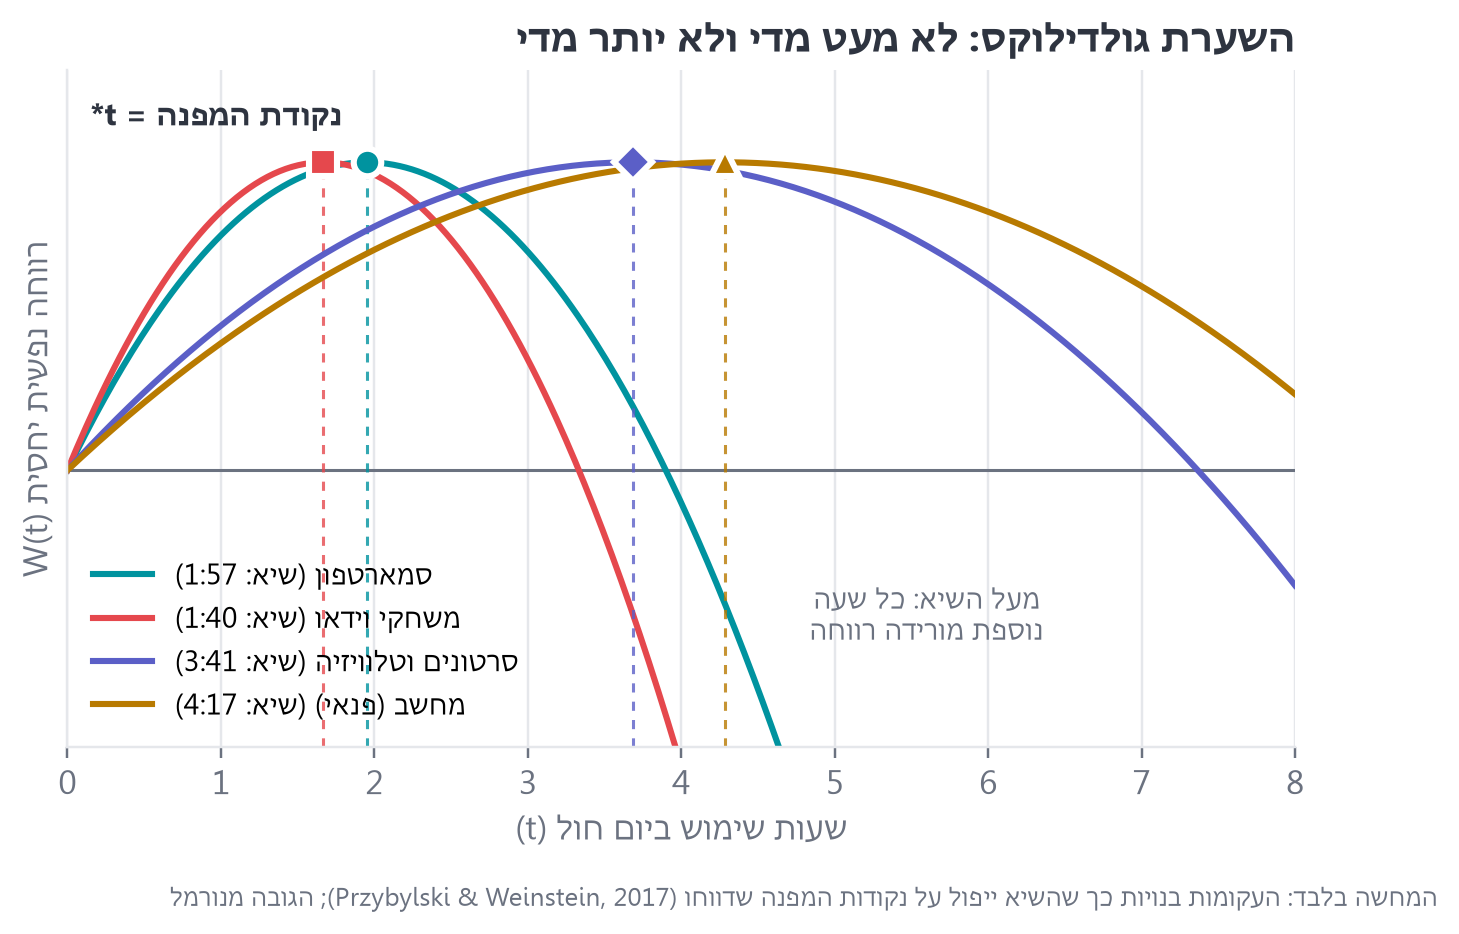
\includegraphics[width=0.92\textwidth]{images/goldilocks.png}
\caption[המחשה של מודל גולדילוקס: נקודת מפנה לכל פעילות]{המחשה של מודל גולדילוקס (משוואה~\ref{eq:goldilocks}): לכל פעילות יש נקודת מפנה $t^{*}$ משלה. נקודות המפנה לימי חול לפי \textcite{przybylski2017}. העקומות בנויות כך שהשיא ייפול על נקודת המפנה, והגובה השווה שלהן הוא נרמול: הן מראות \textbf{איפה} השיא, לא כמה הוא גבוה. האפקט שנמדד בפועל קטן \parencite{orben2019}.}
\label{fig:goldilocks}
\end{figure}
